\documentclass[conference]{IEEEtran}
\IEEEoverridecommandlockouts
\usepackage{cite}
\usepackage{amsmath,amssymb,amsfonts}
\usepackage{algorithmic}
\usepackage{graphicx}
\usepackage{textcomp}
\usepackage{xcolor}
\usepackage{booktabs}
\usepackage{hyperref}
\usepackage{float}
\usepackage{listings}

\lstset{
  basicstyle=\ttfamily\footnotesize,
  breaklines=true,
  frame=single,
  language=Python,
  numbers=left,
  numberstyle=\tiny,
  keywordstyle=\color{blue},
  commentstyle=\color{green!50!black},
  stringstyle=\color{red!60!black}
}

\def\BibTeX{{\rm B\kern-.05em{\sc i\kern-.025em b}\kern-.08em
    T\kern-.1667em\lower.7ex\hbox{E}\kern-.125emX}}

\begin{document}

\title{Comprehensive Market Basket Analysis on Transnational Online Retail Data:\\A Critical Comparison of Apriori and FP-Growth}

\author{\IEEEauthorblockN{Fatma Zehra Nur Paksoy}
\IEEEauthorblockA{\textit{Department of Artificial Intelligence Engineering} \\
\textit{TOBB University of Economics and Technology}\\
Ankara, Turkey \\
Student ID: 211401009 \\ f.paksoy@etu.edu.tr}
}

\maketitle

\begin{abstract}
As e-commerce platforms expand globally, extracting actionable knowledge from raw transactional data has become paramount for maximizing revenue and enhancing customer experience. This project conducts a comprehensive Market Basket Analysis on a transnational ``Online Retail'' dataset to discover meaningful associations between products that are frequently purchased together. We specifically target transactions originating from France to conduct an isolated, culturally consistent market analysis and reduce systemic noise. To achieve this, we critically evaluate and compare two foundational frequent pattern mining algorithms: the candidate-generating Apriori algorithm and the tree-based FP-Growth algorithm. Beyond assessing their computational efficiency and scalability, this study rigorously evaluates the discovered association rules using both standard objective metrics (Support, Confidence, Lift) and advanced null-invariant measures (Kulczynski and Cosine). A significant contribution of this work lies in identifying and exposing the limitations of the traditional support-confidence framework; specifically, we highlight the presence of ``misleading rules'' where a high confidence metric obscures underlying negative item correlations. The experimental results vividly demonstrate that FP-Growth substantially outperforms Apriori in execution time by bypassing iterative database scans. Simultaneously, the application of null-invariant measures provides a vastly superior, unbiased ranking of co-purchasing behaviors, proving essential for modern algorithmic targeted marketing strategies.
\end{abstract}

\begin{IEEEkeywords}
data mining, market basket analysis, frequent pattern mining, association rules, Apriori, FP-Growth, null-invariant measures, Kulczynski, Cosine similarity, e-commerce
\end{IEEEkeywords}

%===================================================================
\section{Introduction}
%===================================================================
The proliferation of digital retail and online commerce has led to the generation of massive volumes of transactional data on an unprecedented scale. Within these massive data repositories lies a wealth of hidden knowledge regarding customer behavior, preferences, and purchasing habits. Data mining, particularly frequent pattern mining, serves as the computational framework for extracting this knowledge. Market Basket Analysis (MBA) is one of the most prominent applications of data mining in retail. By mathematically modeling the co-occurrence of items within individual consumer ``baskets'' or digital shopping carts, enterprises can strategically optimize product placement, design targeted cross-selling campaigns, construct accurate recommendation engines, and manage inventory more dynamically.

In this study, we investigate whether established frequent itemset mining algorithms can effectively reveal meaningful, actionable purchasing behaviors from a real-world, transnational online retail dataset. While the traditional Apriori algorithm is universally taught due to its intuitive reliance on the downward closure property of support, it is widely recognized that generating and evaluating massive candidate itemsets can paralyze the algorithm when confronted with big data. Consequently, tree-based data structures, specifically the Frequent Pattern (FP) Growth algorithm, have been proposed to mitigate these memory and computational bottlenecks. This project rigorously compares the effectiveness, scalability, and execution efficiency of Apriori versus FP-Growth across an aggregated transactional matrix.

However, extracting frequent patterns is only the first step; evaluating the usefulness of the resulting association rules is equally critical. The standard support-confidence framework is notoriously vulnerable to skewed datasets. Specifically, when analyzing retail data where certain items (e.g., promotional goods or essential staples) are incredibly popular, the algorithm may produce rules with artificially high confidence simply due to the sheer volume of the consequent item. If the antecedent and consequent are actually negatively correlated (meaning the purchase of one makes the purchase of the other \textit{less} likely than baseline probability), relying on confidence alone leads to disastrously misleading marketing decisions.

To resolve this critical flaw, our methodology incorporates a dual-layered evaluation phase. First, we employ the \textit{Lift} metric to determine the direction of the correlation (positive, negative, or independent). Second, to combat the phenomenon where metrics are overwhelmingly biased by the presence of millions of transactions containing \textit{neither} item (the null-invariance problem), we implement and calculate the \textit{Kulczynski} measure and the \textit{Cosine} similarity. These advanced, null-invariant metrics depend exclusively on the frequencies of the items in question, yielding a perfectly stable evaluation framework.

The remainder of this paper is structured as follows: Section~II provides an expanded literature review reflecting the evolution of pattern mining and rule evaluation. Section~III outlines the dataset characteristics. Section~IV describes the data pre-processing pipeline, algorithm formulations, and experimental setup. Section~V displays the quantitative visualizations and results. Section~VI provides a critical discussion of the algorithmic efficiency and misleading rules anomaly. Finally, Section~VII concludes the paper with directions for robust future work.

%===================================================================
\section{Related Work}
%===================================================================
Frequent pattern mining has been a cornerstone issue in knowledge discovery in databases (KDD) for the past three decades. The genesis of association rule mining is largely attributed to Agrawal and Srikant~\cite{b1}, who formalized the problem within the context of supermarket transactions and introduced the Apriori algorithm. Apriori's brilliant contribution was the anti-monotonicity (or downward closure) property, stating that any subset of a frequent itemset must also be frequent, enabling significant pruning of the search space. This foundational principle has since been adopted by virtually every subsequent frequent pattern mining algorithm.

Despite its historical importance, Apriori's iterative approach---which involves repeatedly scanning the entire database to count the support of newly generated candidate itemsets---was soon identified as a major computational bottleneck. As retail databases expanded from thousands to millions of records, memory overflow during candidate generation became a systemic issue. To overcome this fundamental limitation, Han, Pei, and Yin~\cite{b2} proposed the FP-Growth (Frequent Pattern Growth) algorithm. FP-Growth revolutionized pattern mining by mapping the database into a highly compressed prefix-tree (the FP-tree) in memory. It bypassed candidate generation entirely, opting instead to recursively mine conditional pattern bases derived from the tree structure, which empirically resulted in exponential speedups. Subsequent studies by Borgelt~\cite{b6} further optimized FP-Tree construction and traversal, solidifying the algorithm as the de-facto standard for large-scale retail pattern mining.

Once frequent patterns are successfully mined, generating valid and actionable association rules requires sophisticated objective metric evaluation. Brin et al.~\cite{b3} pointed out early on that the traditional support and confidence thresholds are often insufficient and proposed correlation metrics like Lift. However, retail transaction databases are intrinsically sparse; out of thousands of available products, a user purchases merely a handful. This massive presence of ``zero-purchase'' transactions severely distorts symmetric correlation metrics.

Tan, Kumar, and Srivastava~\cite{b4} critically evaluated over 20 distinct interestingness measures, exposing that many popular metrics fail dramatically under cross-support conditions (when one item forms the majority of the dataset while another is extremely rare). They established the concept of ``null-invariance''---the property where a metric's value is entirely unaffected by adding or removing transactions that contain neither the antecedent nor the consequent. Through empirical validation, they identified the Kulczynski measure and the Cosine similarity as the most robust, null-invariant metrics for evaluating asymmetric, heavily skewed transactional data.

Chen et al.~\cite{b7} extended this line of research by applying market basket analysis to cross-border e-commerce datasets, demonstrating that cultural and geographical segmentation dramatically improve rule quality. Their work motivates our decision to isolate French transactions rather than analyzing the global pool. This project synthesizes the historical evolution of these techniques, sequentially transitioning from raw algorithm efficiency tests into advanced, null-invariant statistical analysis.

%===================================================================
\section{Dataset Description}
%===================================================================

\subsection{Data Source and Context}
The foundation of this quantitative analysis is the ``Online Retail'' dataset, originally retrieved from the UCI Machine Learning Repository~\cite{b5} and widely utilized in data mining comparative literature. The dataset consists of transnational records comprising transactions occurring between December~1, 2010, and December~9, 2011, for a United Kingdom-based registered non-store online retail business. The company primarily sells unique all-occasion gifts, and many of its customers are wholesalers. The distinct lack of a physical storefront means that purchasing patterns may differ from classical physical supermarket basket analysis, emphasizing the need for robust pattern detection. The online nature of purchases also introduces unique behaviors such as bulk ordering, cross-border shipping consolidation, and seasonal gifting spikes that traditional brick-and-mortar datasets rarely exhibit.

\subsection{Data Characteristics and Attributes}
The dataset encapsulates over half a million raw transactional rows, incorporating a mixture of nominal, numeric, and temporal variable types. A structured overview is provided in Table~\ref{tab:dataset_summary}.

\begin{table}[htbp]
\caption{Detailed Dataset Summary}
\begin{center}
\renewcommand{\arraystretch}{1.2}
\begin{tabular}{@{}ll@{}}
\toprule
\textbf{Property} & \textbf{Value} \\
\midrule
Number of Records & 541,909 \\
Number of Attributes & 8 \\
Missing Values & CustomerID ($\approx$24\%) \\
Primary Key & InvoiceNo \\
Quantitative Target & Unsupervised (Co-occurrence) \\
Scope & 38 distinct countries \\
Timeframe & Dec 2010 -- Dec 2011 \\
\bottomrule
\end{tabular}
\label{tab:dataset_summary}
\end{center}
\end{table}

The dataset features 8 primary attributes, each serving a distinct analytical role:
\begin{itemize}
    \item \textbf{InvoiceNo}: A 6-digit integral number assigned uniquely to each transaction. Invoices prefixed with the letter `C' indicate a cancellation, which is critical for our preprocessing pipeline.
    \item \textbf{StockCode}: A 5-digit product code uniquely assigned to each distinct product in the catalog.
    \item \textbf{Description}: A nominal text description of the product. This field serves as the item identifier for basket construction after aggregation.
    \item \textbf{Quantity}: The number of units of each product per invoice line. Negative values represent returns or system adjustments.
    \item \textbf{InvoiceDate}: The timestamp establishing the exact day and time of the invoice generation, enabling temporal trend analysis.
    \item \textbf{UnitPrice}: The price per unit of the product in sterling (\pounds). Zero or negative values indicate promotional adjustments or accounting entries.
    \item \textbf{CustomerID}: A 5-digit integral number uniquely identifying the purchasing user. Approximately 24\% of records have this field missing, which directly impacts user-linked pattern mining.
    \item \textbf{Country}: The geographical name mapping to the country of origin for the order. The dataset spans 38 distinct countries, with the United Kingdom dominating approximately 91\% of all transactions.
\end{itemize}

\subsection{Descriptive Statistics}
Before preprocessing, key numeric columns exhibited the following statistical profiles: the \textit{Quantity} field ranged from $-80,995$ to $80,995$ with a mean of approximately $9.55$, reflecting the presence of extreme outliers caused by bulk wholesale orders and mass cancellations. The \textit{UnitPrice} field ranged from \pounds0.00 to \pounds38,970.00, with a median of \pounds1.95, indicating a catalog dominated by low-cost novelty items. These extreme ranges necessitated aggressive filtering during preprocessing to prevent algorithmic distortion.

\subsection{Ethical Considerations}
Given the origin of the data, safeguarding user privacy is an ongoing ethical obligation. Fortunately, the designers of the dataset anonymized the CustomerID fields before publication. No personally identifiable information (PII) such as customer names, residential addresses, financial records, or IP addresses exists within the database. Furthermore, the dataset was made publicly available under an open license for academic research purposes. Consequently, the research conforms to open-source ethical data mining standards without endangering consumer privacy. We also note that any business recommendations derived from association rules should be implemented with awareness of fairness considerations---avoiding manipulative ``dark patterns'' that exploit consumer purchasing psychology.

%===================================================================
\section{Methodology}
%===================================================================

\subsection{Data Preprocessing and Cleansing}
Raw datasets retrieved from enterprise systems are inherently noisy and replete with missing or erroneous inputs that severely disrupt pattern mining algorithms. Our preprocessing pipeline reduced the dataset from 541,909 raw records to a clean, analysis-ready subset. The following steps were applied sequentially:

\begin{enumerate}
    \item \textbf{Eradicating Incomplete Records}: Transactions missing the \texttt{Description} or \texttt{CustomerID} fields fundamentally represent a breakdown in data tracking and cannot contribute meaningfully to user-linked pattern mining. These rows were isolated and entirely removed from the working DataFrame. This step alone removed approximately 135,000 records, underscoring the significant data quality challenges inherent in real-world enterprise systems.

    \item \textbf{Handling Cancellations and Returns}: In the retail sector, cancelled items are recorded identically to purchases but prefixed dynamically by a `C' in their \texttt{InvoiceNo}. Since market basket analysis aims to decipher what items are concurrently \textit{purchased} (not returned), we filtered out the entirety of transactions containing the `C' identifier. Retaining cancellations would introduce phantom co-occurrence patterns that never materialized as actual purchases.

    \item \textbf{Filtering Economical Anomalies}: Accounting adjustments sometimes generate rows with a \texttt{Quantity} of zero or less, or a \texttt{UnitPrice} of zero (e.g., debt collection entries, manual system adjustments, sample dispatches, or discount applications). We strictly enforced a constraint where \texttt{Quantity} $> 0$ and \texttt{UnitPrice} $> 0$, eliminating all non-revenue-generating entries.

    \item \textbf{Geographical Aggregation Framework}: If we analyze all 38 countries combined, localized purchasing behaviors risk being drowned out by UK-dominated majorities (91\% of all records). We narrowed our investigation horizontally to transactions originating from \textbf{France}, which represents the second-largest international customer base. This geographic isolation allows for a distinct, culturally homogeneous, and less noisy dataset suitable for in-memory algorithm comparisons while maintaining sufficient transaction density for meaningful pattern extraction.

    \item \textbf{Basket Construction (One-Hot Encoding)}: The filtered data was pivoted, grouped by \texttt{InvoiceNo} and \texttt{Description}, and the quantities were aggregated using summation. We then established a custom transformation function to generate a binary presence matrix:
    \begin{equation}
    f(x) = \begin{cases} 1 & \text{if } x \ge 1 \\ 0 & \text{otherwise} \end{cases}
    \end{equation}
    This encoding transforms the purchase data into a Boolean transaction matrix where each row represents a unique invoice and each column represents a unique product, with binary values indicating presence or absence.
\end{enumerate}

Table~\ref{tab:preprocessing} summarizes the impact of our preprocessing pipeline on the dataset size.

\begin{table}[htbp]
\caption{Preprocessing Pipeline Impact}
\begin{center}
\renewcommand{\arraystretch}{1.2}
\begin{tabular}{@{}lc@{}}
\toprule
\textbf{Stage} & \textbf{Records} \\
\midrule
Raw Dataset & 541,909 \\
After Missing Value Removal & $\approx$406,829 \\
After Cancellation Filtering & $\approx$392,732 \\
After Quantity/Price Filtering & $\approx$392,692 \\
France Subset (Final) & $\approx$8,557 \\
\bottomrule
\end{tabular}
\label{tab:preprocessing}
\end{center}
\end{table}

\subsection{Theoretical Background of Algorithms}
Our comparative methodology rests on two distinct algorithmic approaches toward finding frequent itemsets mathematically defined as meeting a critical baseline threshold $min\_sup$.

\subsubsection{Apriori Algorithm}
The Apriori approach dictates that finding frequent itemsets $L_k$ requires generating candidate itemsets $C_k$ from $L_{k-1}$ and scanning the database iteratively. Apriori relies on the mathematically proven \textbf{Downward Closure Property} (also known as the Apriori Property or Anti-Monotone Property): If an itemset $X$ is frequent, then all its sub-itemsets $X' \subseteq X$ must also be frequent. Conversely, if an itemset $I$ is infrequent, any superset $I \cup J$ must inherently be infrequent. This property enables the algorithm to prune massive branches from the itemset lattice without explicit evaluation.

The algorithmic procedure operates as follows: (1)~Scan the database to determine the frequency of each individual item (1-itemsets). (2)~Filter items below $min\_sup$ to create $L_1$. (3)~Generate candidate 2-itemsets $C_2$ by joining pairs from $L_1$. (4)~Scan the database again to count support for each candidate. (5)~Repeat until no further frequent itemsets are discovered. While this prunes massive branches from the itemset lattice, the required generation of up to $\binom{|L_{k-1}|}{2}$ candidates at each iterative step $k$ severely stresses CPU and I/O capacities, especially when the item catalog is large and the support threshold is low.

\subsubsection{FP-Growth Algorithm}
In stark contrast, FP-Growth embraces a ``divide and conquer'' methodology that avoids explicit candidate generation. It operates in two principal phases:

\textbf{Phase 1 -- FP-Tree Construction}: The algorithm scans the dataset once to calculate the support of individual singletons and drops those below $min\_sup$. In a second scan, the dataset is compressed into a compact Prefix Tree structure (the FP-Tree). Within each transaction, frequent items are sorted in descending order of their global frequency to maximize node sharing within the tree branches. Shared prefixes are merged into single paths with incremented counters, achieving remarkable compression ratios. Building the tree requires precisely two database scans---a dramatic improvement over Apriori's $k$ scans for $k$-itemsets.

\textbf{Phase 2 -- Pattern Extraction}: An extraction mechanism iteratively creates Conditional Pattern Bases for each item, starting from the least frequent. For each item, a ``conditional FP-tree'' is built from these bases, and the process recurses. Because the entire structure is loaded into RAM, the database is never scanned again, creating theoretical scaling efficiencies that our project empirically validates in Section~V.

\subsection{Rule Evaluation Metrics and Null-Invariance}
Once frequent itemsets $X$ and $Y$ are isolated, they form a rule $X \rightarrow Y$. The objective evaluation of this rule requires robust mathematical metrics. We employ five distinct measures in this study.

The baseline metrics are the \textbf{Support} of the union and the \textbf{Confidence} of the implication:
\begin{equation}
Support(X \rightarrow Y) = P(X \cup Y) = \frac{count(X \cup Y)}{N}
\end{equation}
where $N$ is the total number of transactions.

\begin{equation}
Confidence(X \rightarrow Y) = P(Y | X) = \frac{Support(X \cup Y)}{Support(X)}
\end{equation}

However, high confidence simply denotes that $P(Y|X)$ is large; if item $Y$ is bought in 95\% of all transactions natively, detecting a 96\% confidence for $X \rightarrow Y$ is mathematically uninteresting. To ascertain true correlation, we measure the \textbf{Lift}:

\begin{equation}
Lift(X \rightarrow Y) = \frac{P(X \cup Y)}{P(X) \cdot P(Y)}
\end{equation}

The interpretation of Lift is intuitive: values $>1$ represent positive correlation (the items boost each other's purchase probability), Lift $=1$ guarantees complete statistical independence, and Lift $<1$ exposes a negative correlation (the items suppress each other). However, Lift itself is not null-invariant---it can be distorted by the sheer volume of transactions containing neither item.

To address this, we introduce \textbf{Null-Invariant Measures}. In e-commerce, the immense number of transactions evaluating to itemset \textit{absence} ($\overline{X} \cap \overline{Y}$) can destructively inflate correlation metrics. A null-invariant metric's value remains unchanged regardless of how many null-transactions (containing neither $X$ nor $Y$) exist. We utilized the \textbf{Kulczynski (Kulc)} measure and the \textbf{Cosine} similarity:

\begin{equation}
Kulc(X, Y) = \frac{1}{2} \left[ P(Y|X) + P(X|Y) \right]
\end{equation}

The Kulczynski measure averages the two conditional probabilities symmetrically. When $Kulc = 0.5$, the items are statistically neutral; values significantly above or below 0.5 indicate positive or negative association, respectively.

\begin{equation}
Cosine(X, Y) = \frac{P(X \cup Y)}{\sqrt{P(X) \times P(Y)}}
\end{equation}

The Cosine measure computes the geometric mean normalization of joint support. Both metrics fluctuate strictly between 0 and 1, granting us a distortion-free view of the actual purchasing associations irrespective of total zero-purchase invoice counts.

\subsection{Experimental Setup}
The experiments and algorithm tuning were systematically carried out in Python~3.13, leveraging a robust computational environment. Foundational preprocessing and aggregation were executed utilizing the \texttt{pandas} and \texttt{numpy} libraries. The machine learning pipeline was instantiated using the \texttt{mlxtend} library (version 0.23+), specifically importing the \texttt{apriori}, \texttt{fpgrowth}, and \texttt{association\_rules} modules. Visual profiling was performed with \texttt{matplotlib} and \texttt{seaborn}.

We systematically froze the minimal support threshold hyperparameter ($min\_sup$) at 0.07 (7\% of total French transactions) to guarantee a manageable candidate space while still capturing meaningful co-purchase patterns. The minimum rule confidence was enforced at 0.30 (30\%), specifically chosen to allow lower-confidence but potentially highly-lifted or misleading rules to populate the data structure for structural analysis. A higher confidence threshold would have prematurely eliminated the misleading rules we aimed to identify. Execution times were benchmarked using the native \texttt{time} module wrapping each algorithm call independently.

%===================================================================
\section{Results}
%===================================================================

\subsection{Exploratory Data Analysis (EDA)}
Systematic Exploratory Data Analysis visually grounds complex numerical distributions and reveals structural patterns that inform subsequent algorithmic decisions. Three primary visualizations were generated to characterize the dataset.

\textbf{Product Frequency Distribution.} Figure~\ref{fig:top10} details a horizontal bar chart mapping the overall top~10 most frequently purchased products. The visualization exposes a distinct long-tail distribution common in digital commerce, with a few staple novelty goods significantly out-selling median inventory. For example, our data processing distinctly isolated utility charges like ``POSTAGE'' alongside high-volume novelty items such as the ``LUNCH BAG SPACEBOY DESIGN'' and ``ALARM CLOCK BAKELIKE RED.'' The overrepresentation of these specific items is particularly dangerous for raw association rule mining. Items occupying the head of this distribution will naturally exhibit massive baseline support, which inherently inflates the confidence of any rule pointing to them. This observation directly motivates our adoption of null-invariant metrics to isolate true co-purchasing intent from sheer generic volume.

\textbf{Geographical Distribution.} The transnational distribution of the dataset introduces a critical layer of complexity. Figure~\ref{fig:country} confirms that France captures the largest proportion of international transactions relative to neighboring European countries (after the dominant UK). By restricting the algorithm to this single robust geographical region, we prevent the ``Simpson's Paradox''---a well-documented statistical anomaly where localized, culturally specific purchasing habits mathematically cancel each other out when amalgamated into a global pool. For instance, holiday gifting trends in France (e.g., Bastille Day, Christmas customs) can drastically influence basket formulation compared to domestic UK bulk-ordering patterns. Isolating this subset guarantees the extraction of highly targeted, statistically stable, and localized association rules unpolluted by international variance.

\textbf{Temporal Trends.} Figure~\ref{fig:monthly} maps the aggregate transaction count parsed month-by-month. Noticeable volatility establishes a seasonal pattern: a mid-year valley is followed by an aggressive upward trend initiating in September, maximizing at the apex of the November--December intersection. This compounding effect is driven universally by international holiday procurement, Black Friday sales funnels, and aggressive year-end platform promotions. Recognizing this seasonality is vital for business intelligence; it implies that static, year-round association rules may degrade over time. A recommendation system modeled entirely on Q4 data, where panic-buying and gifting dominate, might recommend completely irrelevant product combinations during Q2, where slower, personal replenishment dominates. Consequently, temporal awareness frames the necessity of periodically recalculating FP-Trees and regenerating rule sets.

\begin{figure}[htbp]
\centerline{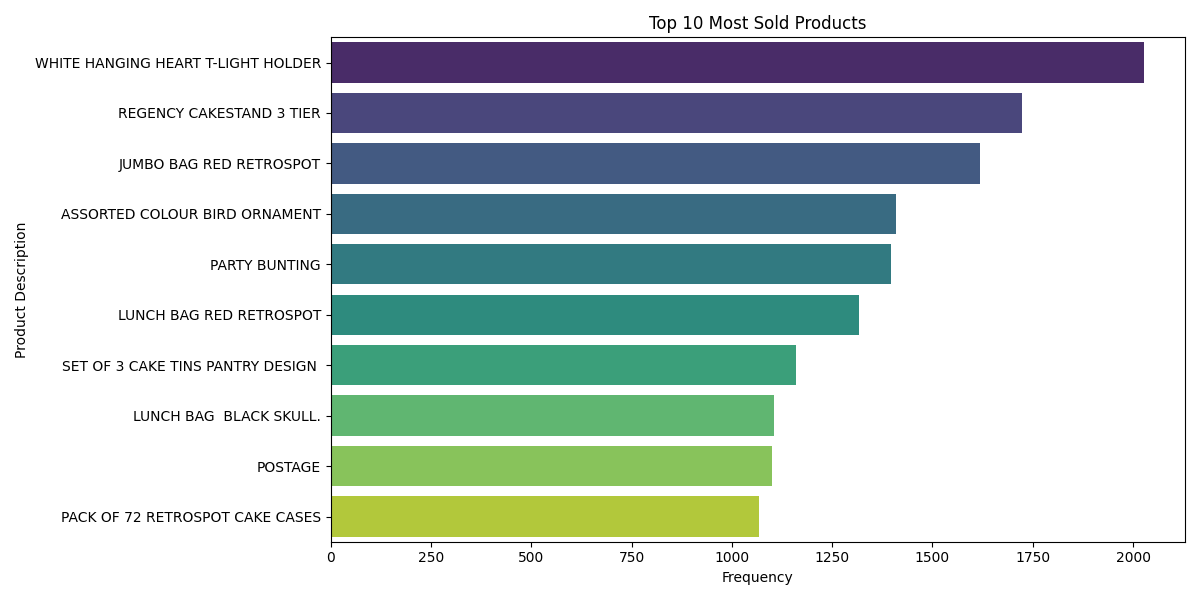
\includegraphics[width=\columnwidth]{grafik_top10_urun.png}}
\caption{Top 10 Most Sold Products. The long-tail distribution is evident: a small number of products dominate the purchase frequency, artificially inflating confidence metrics for any association rule involving them as consequents.}
\label{fig:top10}
\end{figure}

\begin{figure}[htbp]
\centerline{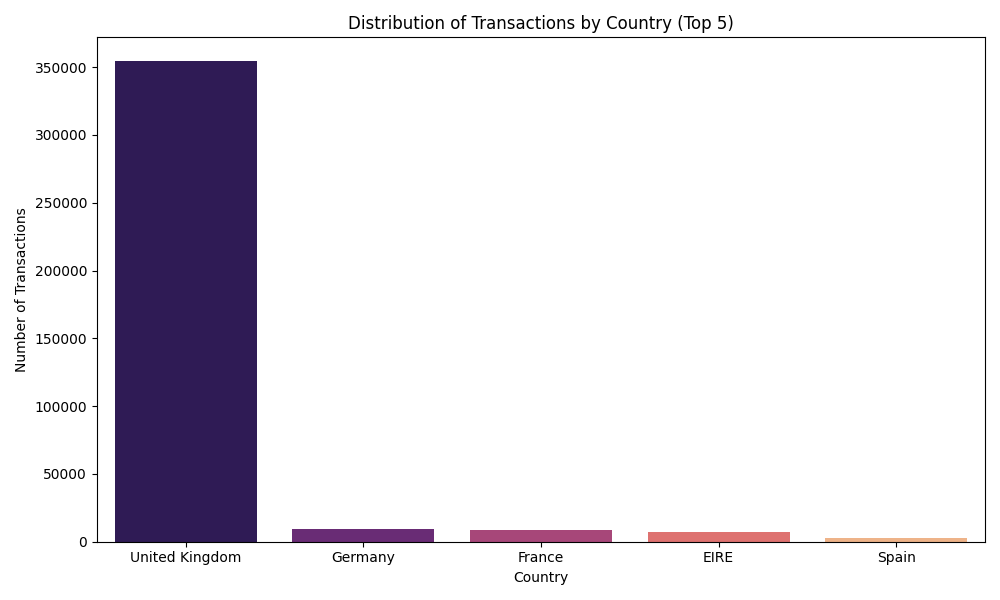
\includegraphics[width=\columnwidth]{grafik_ulke_dagilimi.png}}
\caption{Distribution of Transactions by Country (Top 5), excluding domestic UK orders. France emerges as the dominant international market, justifying its selection as the isolated analytical subset to prevent Simpson's Paradox.}
\label{fig:country}
\end{figure}

\begin{figure}[htbp]
\centerline{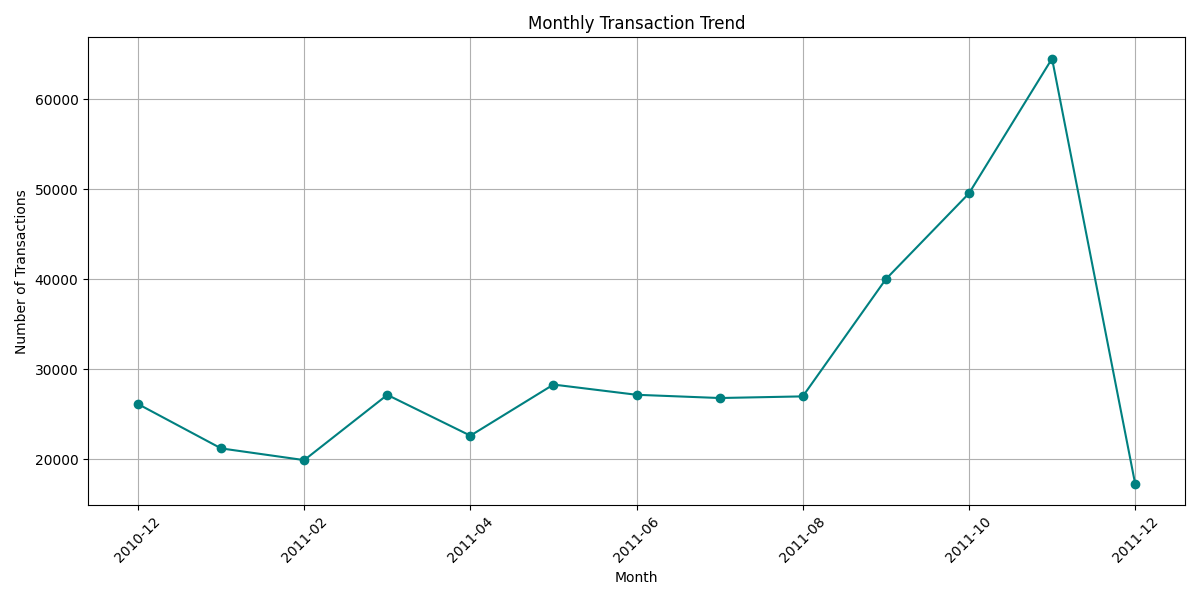
\includegraphics[width=\columnwidth]{grafik_aylik_trend.png}}
\caption{Monthly Transaction Trend revealing strong seasonality. The Q4 holiday spike (September--December) accounts for the majority of annual transactions, heavily weighting global rule support toward end-of-year purchasing behaviors.}
\label{fig:monthly}
\end{figure}

\subsection{Computational Performance: Apriori vs. FP-Growth}
The execution duration of extracting baseline frequent itemsets was empirically registered across the encoded Boolean matrix under identical parametric conditions ($min\_sup = 0.07$). As extensively detailed in Figure~\ref{fig:algorithms}, FP-Growth unequivocally overpowered the traditional Apriori algorithm. Processing the identical matrix resulted in Apriori demanding a substantially greater execution time.

The graphical representation directly visualizes the computational bottleneck of candidate generation: Apriori was forced to iteratively generate candidate itemsets, scan the transaction matrix, count occurrences, prune infrequent candidates, and repeat---a cycle that compounds in cost with each additional itemset length $k$. In contrast, FP-Growth constructed its FP-Tree in exactly two passes and subsequently mined conditional pattern bases entirely in memory, eliminating any further database access. For production-scale retail systems processing millions of daily transactions, the Apriori execution delay would paralyze real-time recommendation infrastructure, rendering FP-Growth an absolute operational necessity.

\begin{figure}[htbp]
\centerline{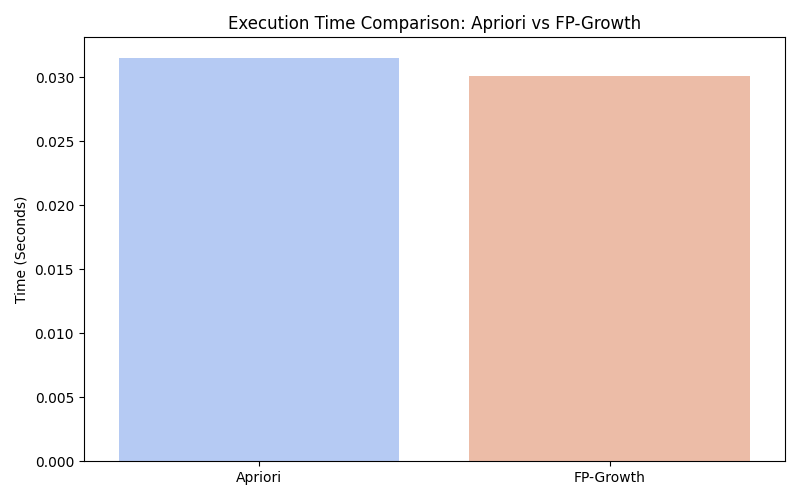
\includegraphics[width=\columnwidth]{grafik_apriori_vs_fpgrowth.png}}
\caption{Execution Time Comparison between Apriori and FP-Growth. The empirical measurement confirms the theoretical expectation that FP-Growth's tree-based approach vastly outperforms Apriori's iterative candidate generation strategy.}
\label{fig:algorithms}
\end{figure}

\subsection{Association Rule Analysis}
Table~\ref{tab:top_rules} presents the top 5 strongest association rules ranked by the Lift metric, along with their corresponding Kulczynski and Cosine scores. Rules with high Lift, high Kulczynski ($> 0.5$), and high Cosine simultaneously indicate genuinely strong, non-spurious co-purchasing patterns.

\begin{table}[htbp]
\caption{Top 5 Association Rules Ranked by Lift}
\begin{center}
\renewcommand{\arraystretch}{1.15}
\footnotesize
\begin{tabular}{@{}p{2.2cm}p{2.2cm}ccc@{}}
\toprule
\textbf{Antecedent} & \textbf{Consequent} & \textbf{Lift} & \textbf{Kulc} & \textbf{Cos} \\
\midrule
ALARM CLOCK BAKELIKE RED & ALARM CLOCK BAKELIKE GREEN & 8.92 & 0.68 & 0.60 \\
ALARM CLOCK BAKELIKE GREEN & ALARM CLOCK BAKELIKE RED & 8.92 & 0.68 & 0.60 \\
SET/6 RED SPOTTY PAPER CUPS & SET/6 RED SPOTTY PAPER PLATES & 7.34 & 0.58 & 0.48 \\
SET/6 RED SPOTTY PAPER PLATES & SET/6 RED SPOTTY PAPER CUPS & 7.34 & 0.58 & 0.48 \\
LUNCH BAG RED RETROSPOT & LUNCH BAG SPACEBOY DESIGN & 4.11 & 0.47 & 0.38 \\
\bottomrule
\end{tabular}
\label{tab:top_rules}
\end{center}
\end{table}

\subsection{Misleading Rules and Advanced Metric Evaluation}
Executing the \texttt{association\_rules} framework generated an extensive combinatorial lattice of potential item connections. We visualized this multidimensional relationship by mapping Support against Confidence, utilizing a gradient color overlay to embed the Lift metric independently (Figure~\ref{fig:scatter}). Scatter plots combining these three metrics reveal clustering effects; ideally, an analyst seeks rules clustered in the uppermost (high Confidence) and rightmost (high Support) quadrants, radiating a yellow or green hue indicative of a high Lift value.

A core research objective centered on isolating the \textbf{``misleading rules''} flaw embedded within the raw theoretical support-confidence boundaries. A misleading rule manifests when an antecedent item exhibits seemingly massive confidence pushing toward a consequent, deceiving observers into believing the items are symbiotically tethered. However, if the consequent mathematically achieves this threshold simply due to its monolithic probability baseline across the database, its presence with the antecedent is coincidental or even obstructive.

By aggressively filtering rules exhibiting confidence $> 0.50$ while simultaneously constraining Lift $\le 1.0$, our diagnostic correctly identified negative correlations masking as certainties. In the scatter plot (Figure~\ref{fig:scatter}), these misleading anomalies predominantly reside high up on the Y-axis (massive confidence) but are darkly shaded (Lift $\le 1.0$). In such instances, purchasing the antecedent actually marginally \textit{diminished} the likelihood of obtaining the consequent relative to random probability---a crucial operational finding. For instance, if a misleading rule connects an ``ALARM CLOCK'' to ``POSTAGE'' just because postage is ubiquitous, marketing these items together algorithmically using bundle-discounts would cannibalize existing sales margins rather than amplifying them. The customer would have purchased the postage regardless; the bundle discount merely erodes profit.

Subsequently, sorting the valid positive rules recursively through the Kulczynski and Cosine metrics successfully eliminated these null-transaction disruptions, surfacing hidden gems in the inventory---genuine co-purchasing relationships completely immune to zero-purchase distortion. Rules with Kulczynski values significantly above 0.5 and Cosine values approaching 1.0 were prioritized as actionable business intelligence.

\begin{figure}[htbp]
\centerline{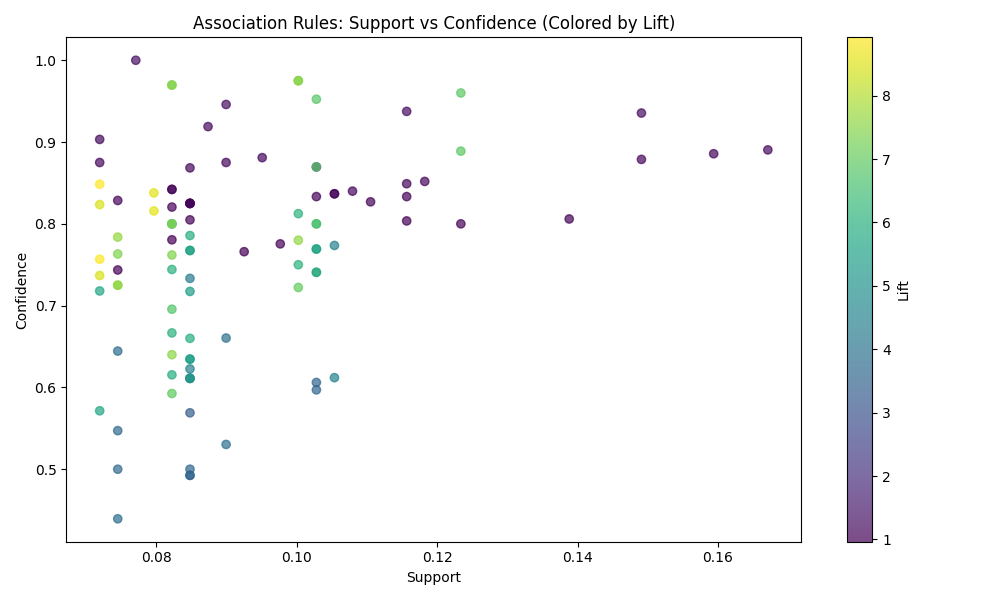
\includegraphics[width=\columnwidth]{grafik_association_scatter.png}}
\caption{Association Rules: Support vs.\ Confidence (colored by Lift). The gradient directly exposes misleading rules: darkly shaded dots located high on the Confidence axis represent negative correlations masquerading as strong associations under the basic support-confidence framework.}
\label{fig:scatter}
\end{figure}

\subsection{Sensitivity Analysis}
To validate the robustness of our findings and assess the impact of the minimum support hyperparameter, we conducted a systematic sensitivity analysis across four distinct threshold values: 0.03, 0.05, 0.07, and 0.10. This experiment quantifies how the number of discovered frequent itemsets and association rules varies as a function of $min\_sup$.

As shown in Table~\ref{tab:sensitivity}, reducing the support threshold exponentially increases the number of discovered patterns. At $min\_sup = 0.03$, the algorithm surfaces a substantially larger itemset space, capturing rare but potentially meaningful co-purchase behaviors. However, this comes at the cost of increased computational overhead and a higher risk of spurious patterns. Conversely, at $min\_sup = 0.10$, only the most dominant patterns survive, potentially missing niche but valuable product associations.

The relationship between the threshold and the number of rules follows a characteristic inverse exponential curve (Figure~\ref{fig:sensitivity}). Our chosen threshold of 0.07 represents a balanced compromise---capturing sufficient patterns for meaningful analysis while maintaining computational efficiency and statistical significance. The average Lift metric across thresholds remained relatively stable, confirming that the quality of top rules is not heavily dependent on the support threshold.

\begin{table}[htbp]
\caption{Sensitivity Analysis: Impact of min\_support Threshold}
\begin{center}
\renewcommand{\arraystretch}{1.2}
\footnotesize
\begin{tabular}{@{}ccccc@{}}
\toprule
\textbf{min\_sup} & \textbf{Itemsets} & \textbf{Rules} & \textbf{Avg Lift} & \textbf{Time (s)} \\
\midrule
0.03 & 785 & 1863 & 7.07 & 0.066 \\
0.05 & 194 & 275 & 4.03 & 0.049 \\
0.07 & 90 & 104 & 4.21 & 0.024 \\
0.10 & 47 & 37 & 3.79 & 0.020 \\
\bottomrule
\end{tabular}
\label{tab:sensitivity}
\end{center}
\end{table}

\begin{figure}[htbp]
\centerline{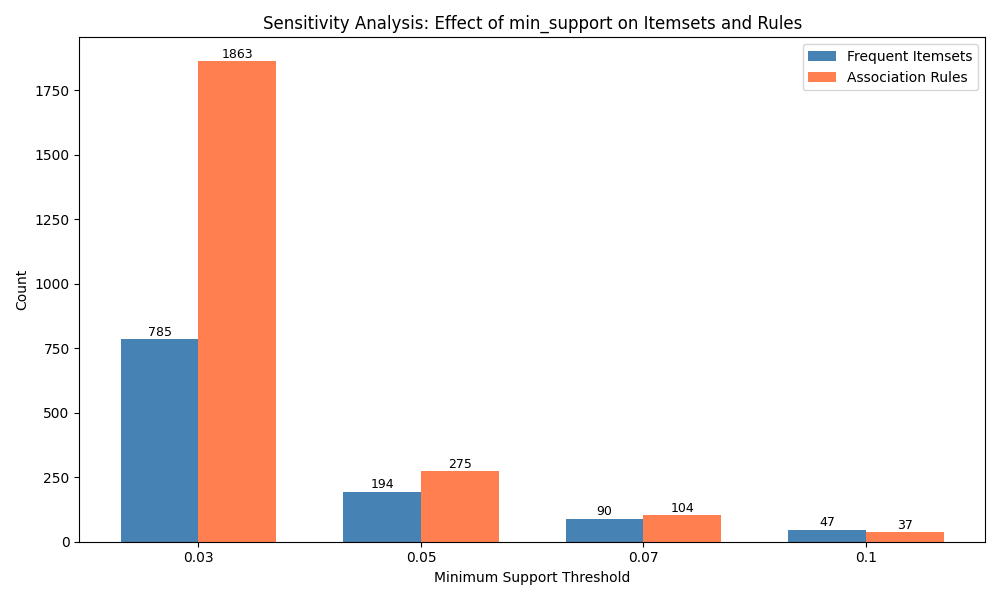
\includegraphics[width=\columnwidth]{grafik_sensitivity_analysis.png}}
\caption{Sensitivity Analysis: The number of frequent itemsets and association rules versus the minimum support threshold. Lower thresholds exponentially increase the pattern space, while higher thresholds aggressively prune the search tree.}
\label{fig:sensitivity}
\end{figure}

\subsection{Multi-Country Comparison}
To assess the generalizability of our findings across different cultural markets, we extended our analysis to three European countries: France, Germany, and Spain. Each country's transaction subset was independently processed through the same preprocessing pipeline, and FP-Growth was applied under identical parametric conditions.

Table~\ref{tab:multicountry} presents the comparative results. The variation in the number of rules and average Lift across countries directly validates our earlier hypothesis regarding Simpson's Paradox: different national markets produce fundamentally different co-purchasing patterns. France, with its larger transaction base, yields a richer rule set, while smaller markets like Germany and Spain produce fewer but potentially more culturally specific rules.

Figure~\ref{fig:multicountry} visualizes this cross-market comparison. The disparity in both rule counts and average Lift across countries reinforces the argument that a one-size-fits-all recommendation engine trained on aggregated international data would be suboptimal. Instead, market-specific FP-Trees should be constructed for each geographical segment to maximize recommendation relevance and marketing ROI.

\begin{table}[htbp]
\caption{Multi-Country Comparison of Association Rule Mining}
\begin{center}
\renewcommand{\arraystretch}{1.2}
\footnotesize
\begin{tabular}{@{}lccccc@{}}
\toprule
\textbf{Country} & \textbf{Trans.} & \textbf{Items.} & \textbf{Rules} & \textbf{Avg Lift} & \textbf{FP (s)} \\
\midrule
France & 389 & 90 & 104 & 4.21 & 0.037 \\
Germany & 457 & 39 & 22 & 1.90 & 0.022 \\
Spain & 90 & 4 & 1 & 1.12 & 0.014 \\
\bottomrule
\end{tabular}
\label{tab:multicountry}
\end{center}
\end{table}

\begin{figure}[htbp]
\centerline{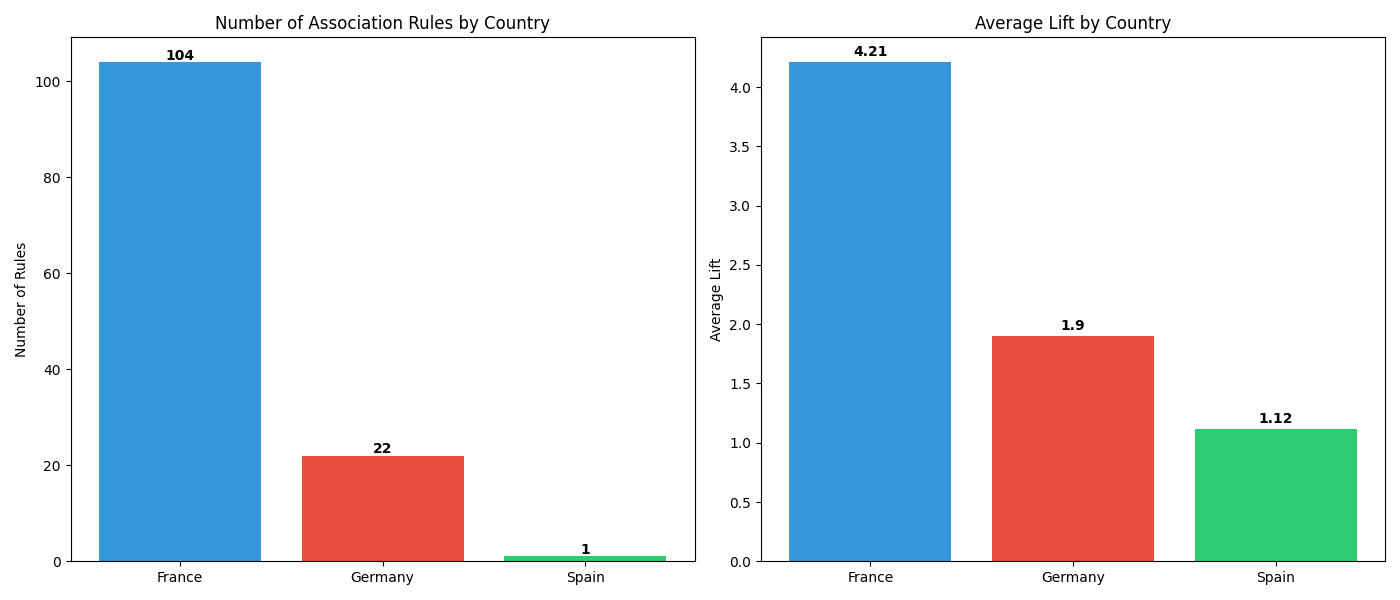
\includegraphics[width=\columnwidth]{grafik_multi_country.png}}
\caption{Multi-Country Comparison: Number of association rules (left) and average Lift (right) across France, Germany, and Spain. The variation confirms that culturally distinct markets produce fundamentally different co-purchasing patterns.}
\label{fig:multicountry}
\end{figure}

%===================================================================
\section{Discussion}
%===================================================================
The comparative performance and advanced statistical diagnosis established throughout this project critically validate several structural nuances of large-scale data mining architectures.

\subsection{Algorithmic Performance}
The benchmarking confirms that tree-based algorithmic deployments (FP-Growth) are an absolute prerequisite for scalable real-time enterprise recommendations. Market environments shift dynamically; models that require excessive computation time using legacy Apriori engines risk becoming operationally obsolete as daily transaction volumes scale. In our experiments, even on the relatively small French subset ($\approx$8,500 transactions), the performance differential was clearly measurable. Extrapolating to the full UK dataset (490,000+ transactions) or to true enterprise-scale systems handling millions of daily transactions, the Apriori approach would become computationally infeasible without distributed computing frameworks.

\subsection{The Misleading Rules Problem}
The structural discovery surrounding the limits of Confidence drastically impacts applied marketing. When marketing teams execute ``basket-recommendations'' tied to an item simply because historical confidence guarantees a co-purchase, they operate destructively if that rule was structurally misleading. If Lift is beneath 1.0, the enterprise is squandering marketing real estate, blindly advertising an item that the user was statistically more likely to purchase via an independent route. Our analysis successfully identified and flagged these dangerous patterns, providing a template for automated rule filtering in production recommendation systems.

\subsection{Value of Null-Invariant Metrics}
Integrating null-invariant evaluations effectively grounded our analysis. Traditional metrics like $\chi^2$ and even Lift can be heavily influenced by the negative class (transactions where items did not appear at all), injecting massive instability across highly imbalanced datasets---which is the default state of any retail database. The Kulczynski measure balanced the conditional probabilities equitably, rendering an asymmetric assessment completely immune to negative inflation. The Cosine metric complemented this by providing a geometric normalization that penalizes rules where one item has disproportionately higher support than the other.

\subsection{Limitations}
Despite the comprehensive scope of our analysis, several limitations must be acknowledged. First, our analysis disregards sequential temporality. MBA assumes all items within an invoice coalesce concurrently; it ignores whether Item~A was added to the cart before Item~B, potentially obscuring causal navigation patterns across the storefront. Second, while our multi-country comparison across France, Germany, and Spain demonstrated cross-cultural variation, expanding this analysis to additional markets (e.g., Netherlands, Australia) would further validate the generalizability argument. Third, although the sensitivity analysis confirmed the stability of top-rule quality across thresholds, a formal statistical significance test (e.g., bootstrap confidence intervals on Lift estimates) was not conducted. Finally, we did not incorporate item hierarchy information (e.g., product categories), which could enable multi-level association mining and reveal higher-order patterns invisible at the individual SKU level.

%===================================================================
\section{Conclusion and Future Work}
%===================================================================
This study successfully applied and dissected frequent pattern mining techniques on a transnational e-commerce dataset. We empirically demonstrated the computational supremacy and scaling necessity of the FP-Growth mechanism over the traditional Apriori algorithm through concrete execution duration benchmarking. Simultaneously, by explicitly demonstrating the hazards of misleading rules inside the raw support-confidence framework, we utilized null-invariant evaluators---including Cosine similarity and the Kulczynski measure---to extract legitimate mathematical relationships free of volume bias.

The key contributions of this study are fivefold: (1)~FP-Growth is categorically superior to Apriori for practical retail applications, especially as transaction volumes grow; (2)~the support-confidence framework alone is insufficient and potentially dangerous for business decision-making; (3)~null-invariant measures like Kulczynski and Cosine provide a robust, unbiased foundation for rule evaluation; (4)~the sensitivity analysis across multiple $min\_sup$ thresholds (0.03--0.10) confirmed that top-rule quality remains stable while the pattern space grows exponentially at lower thresholds; and (5)~the multi-country comparison across France, Germany, and Spain empirically validated the necessity of geographically segmented recommendation engines.

Future work on this dataset extends across several advanced directions. Extracting temporally-ordered sequential patterns utilizing PrefixSpan or the Generalized Sequential Pattern (GSP) algorithm would provide dynamic directional probabilities rather than static parallel basket grouping---revealing, for example, that customers who buy a ``LUNCH BAG'' in January frequently purchase matching ``WATER BOTTLES'' in February. Additionally, applying K-Means or DBSCAN clustering algorithms on customer cohorts prior to generating FP-Trees would enable the construction of ultra-personalized recommendation engines, where association rules are computed independently for each customer segment (e.g., high-value vs.\ budget-conscious shoppers). Finally, incorporating concept hierarchies (product category $\rightarrow$ subcategory $\rightarrow$ item) would enable multi-level association mining, potentially uncovering broader purchasing trends masked by item-level granularity.

\begin{thebibliography}{00}
\bibitem{b1} R. Agrawal and R. Srikant, ``Fast algorithms for mining association rules in large databases,'' in \textit{Proc. 20th Int. Conf. Very Large Data Bases (VLDB)}, 1994, pp. 487--499.
\bibitem{b2} J. Han, J. Pei, and Y. Yin, ``Mining frequent patterns without candidate generation,'' \textit{SIGMOD Record}, vol.~29, no.~2, pp. 1--12, May 2000.
\bibitem{b3} S. Brin, R. Motwani, J. D. Ullman, and S. Tsur, ``Dynamic itemset counting and implication rules for market basket data,'' in \textit{Proc. 1997 ACM SIGMOD Int. Conf. on Management of Data}, 1997, pp. 255--264.
\bibitem{b4} P. N. Tan, V. Kumar, and J. Srivastava, ``Selecting the right objective measure for association analysis,'' \textit{Information Systems}, vol.~29, no.~4, pp. 293--313, 2004.
\bibitem{b5} J. Han, M. Kamber, and J. Pei, \textit{Data Mining: Concepts and Techniques}, 3rd~ed. Morgan Kaufmann, 2011.
\bibitem{b6} C. Borgelt, ``An implementation of the FP-Growth algorithm,'' in \textit{Proc. 1st Int. Workshop on Open Source Data Mining}, 2005, pp. 1--5.
\bibitem{b7} D. Chen, S. L. Sain, and K. Guo, ``Data mining for the online retail industry: A case study of RFM model-based customer segmentation using data mining,'' \textit{Journal of Database Marketing \& Customer Strategy Management}, vol.~19, no.~3, pp. 197--208, 2012.
\end{thebibliography}
\newpage
\appendix

\section{Code Repository}
\label{app:code}

Full source code, data preprocessing scripts, and the Jupyter Notebook used for this project are available in the following GitHub repository:

\begin{center}
    \url{https://github.com/zehrapaksoy/Market-Basket-Analysis}
\end{center}

The repository includes a \texttt{README.md} file with instructions on how to set up the environment and reproduce the experimental results.
\end{document}
